\chapter{Design of the Controller}
\label{chap:controller}
This chapter is focused on the controller system of the Media-Online Management system. The controller system is the hand and mouth of the MOM system. Handling the every day use of MOM system as activating and restricting users from media devices.\newline
This chapter is focused on the controller of the Media-Online Management system. The controller consist of a tag reader and power control device which is disgusted in this chapter but when mentioning controller both is implied. \newline
The design and functionality of the prototype controller will be presented in parallel to the designed end product. \newline

\section{Product Design}

The product design section is the vision of the system as a finised product. Figure \ref{fig:Power&Tagdevice} is the illustation of the embedded system called the controller system. The controller system is connected to the server though a wifi connection to insure that a ethernet outlet don't need to be a every media devise.  
The controller is two devices, detection device and power control device.

\begin{figure}[h]
	\centering
		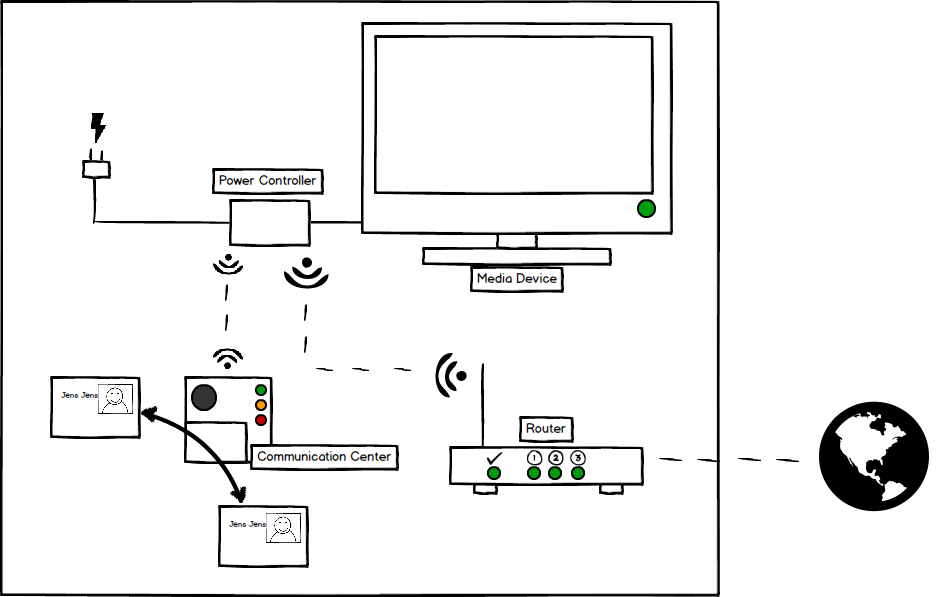
\includegraphics[width=1.00\textwidth]{images/Power&Tagdevice.png}
	\caption{Rich picture for Powercontrol and Tag reader}
	\label{fig:Power&Tagdevice}
\end{figure}

Detection device reads user tags when swiped over the detector device. This device is separated from the power control device to increase user friendliness. The power control device will be placed on the power cable to the media device will that not always be as accessible for the use if one want to scan a tag. Therefor shall the detection device often be placed infront of the media device to give the user friendliness.\newline
The other device is a powercontrol device which is located on the powerline to the media device and turns on and off the electricity when needed.\newline
The powercontrol device(PCD) is the brain of the two devices and is therefore to monitor the time usage of the media. It should also communicate with the server and detection device. \newline
The detection device(DD) should also inform the user who is trying to activate a media of whether the activation has been approved or declined by the server.
%The detection device(DD) also works as an information communicator to the user, on the state of the connection to the server about acceptance/decline of log-in. \newline    

\subsection{Senario Design}
\label{subsec:senarioD}

The system has been designed on multiple scenarios and the criteria of communication to the server and user. The flow chart \ref{} is an overview of the action and communication between server, the controller system and user. The flow chart illustrat the controller system:

\begin{itemize}	
	\item Register user tags and get user rights from server. 
	\item Adminstrat user rigths according to server information.
	\item Moniter the connection wifi to server and handele the exseption op disconnected. 
	\item Regulate the power to a device recording to senario.
	\item Manage the time usaged and user restigtions.
	\item Communicat system status to user.
\end{itemize}

\fixme{indsæt Flowcart af systemet}

The development was done by asking and answer questions to the system in different senarios.\newline
The flow chart is a combined answer here of. \newline

\textbf{Setting up and turning on the system.} \newline
In the final design the PCD will receive the information about the WiFi connection from USB drive.
If the information on the USB is wrong or not received then a restart button is included to redo the procedure.  \newline
The PCD will then connect to the WiFi network and add the controller to the database in his MOM system. If the connection is not found a message is send to the DD. \newline 
DD indicates that there is no connection by showing a constant red light. The communication protocol can be found in the appendix \vref{appen:lights}.\newline When the connection is established then the DD is ready to read user tags.\newline

However, this design will not be implemented in this project. Instead there is a wired connection to the internet and the controller need to be manually added into the database.

\textbf{Detection of connection issues and status changes.} \newline
The connection to the sever is tested by a routine call every five minutes from the PCD to the server. In this call the PCD will receive information on when the media should shutdown based on a rule or the user's remaining time. This insures that if any changes in the remaining time or the rules which will influences when the media should shut down then it will still be handled.
%This insure that there is a connection each five minutes and if any changes in rules or in the time the user may spend on the media. 
In between those calls the PCD will check for a tag from the DD. If the PCD is disconnected from the server that is informed to the DD and to the user.  \newline
	
\textbf{Logon/logoff media divice.} \newline
When a tag is read by the DD the PCD will receive the tag id which is then formed into a log-in message and send to the web servers API. however this is only if no one ready is logged on the media device in the MOM system. The PCD will then get a message about whether the user has permission to use the media from the API. If the user has permission then the PCD should direct power to the media, then save the tag id in local memory and receive the remaining time from the API. The DD should indicate whether the user is approved to use the media.\newline 
To log-off the user will swipe ones user tag again and the PCD receive the same tag id that is stored in the local memory. The PCD will then switch off the power to the media and send a log-off message to the API. \newline
If another user wants to take over the usage of the media then the PCD should try to log-in with the new tag. If this is declined then the DD should then signal this and keep the old user logged on. If it is accepted then the server should overwrite the previous user and PCD will receive the information for the new user with out turning the power off and then on again.\newline 
The functionality of switch users is not implementet in the current prototype.\newline

\textbf{Server disconnection under use.} \newline
A disconnection from the server is either found under the regular status call after each five minutes or at a log-on/log-off call. A disconnection will lock the device so only the current user can use the media until the PCD is reconnected with the server. The server discovers the lack of connection when there have not been a status call from the device in five minutes. The disconnection is translated to a log-off the media at the server side. 
The user will not be logged off by the controller but will be able to use his time according to the last status. If the user want to log-off in a period where there is a disconnection a time stamp is saved and will be sent to the server when the connection is reestablished. The media can also first be used again when the connection is reestablished. 
This procedure have the advantage that the user will not have to cut off the media in use if the connection is unstable. The user will also be able to use a another media with connection to the server.
The disadvantage is that the user has the possible to exceed the time restriction if there has been a change in the rules or the user's remaining time. \newline
The implemtation of exseption of disconnection in prototype is not as the descriped above. \newline 
	